\begin{figure}[h!]
	\centering 
	
	


\tikzset{every picture/.style={line width=0.75pt}} %set default line width to 0.75pt        

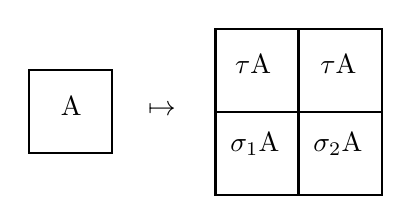
\begin{tikzpicture}[x=0.75pt,y=0.75pt,yscale=-1,xscale=1]
	%uncomment if require: \path (0,300); %set diagram left start at 0, and has height of 300
	
	%Shape: Square [id:dp2023056445996656] 
	\draw   (80,130) -- (120,130) -- (120,170) -- (80,170) -- cycle ;
	%Shape: Square [id:dp7368055726038727] 
	\draw   (170,110) -- (210,110) -- (210,150) -- (170,150) -- cycle ;
	%Shape: Square [id:dp2426334503608445] 
	\draw   (170,150) -- (210,150) -- (210,190) -- (170,190) -- cycle ;
	%Shape: Square [id:dp48040422500928703] 
	\draw   (210,110) -- (250,110) -- (250,150) -- (210,150) -- cycle ;
	%Shape: Square [id:dp2369707217947341] 
	\draw   (210,150) -- (250,150) -- (250,190) -- (210,190) -- cycle ;
	
	% Text Node
	\draw (175.67,158.67) node [anchor=north west][inner sep=0.75pt]   [align=left] {$\displaystyle \sigma _{1}$A};
	% Text Node
	\draw (215.67,158.67) node [anchor=north west][inner sep=0.75pt]   [align=left] {$\displaystyle \sigma _{2}$A};
	% Text Node
	\draw (94,141) node [anchor=north west][inner sep=0.75pt]   [align=left] {A};
	% Text Node
	\draw (136,145.4) node [anchor=north west][inner sep=0.75pt]    {$\mapsto $};
	% Text Node
	\draw (178,121) node [anchor=north west][inner sep=0.75pt]   [align=left] {$\displaystyle \tau $A};
	% Text Node
	\draw (219,121) node [anchor=north west][inner sep=0.75pt]   [align=left] {$\displaystyle \tau $A};
	
	
\end{tikzpicture}
\end{figure}